\documentclass[a4paper,12pt]{report}

\nocite{*}

\newcommand{\nameInitial}{
    \textcolor{black}{G. Allen}
}
\newcommand{\nameFull}{
    \textcolor{black}{Gary Allen}
}
\newcommand{\stNumber}{
    \textcolor{black}{23905093}
}
\newcommand{\myDate}{\textcolor{black}{\today}
}
\newcommand{\signature}{frontmatter/figures/Signature}

% Page layout
\usepackage[left=2.2cm,right=2.2cm,top=2.2cm,bottom=2.2cm]{geometry}

% Figures
\usepackage[margin=\the\parindent,small,bf,sf]{caption}
\usepackage{graphicx}
\usepackage{pdfpages}
\setlength{\abovecaptionskip}{7.5pt}  % spacing above and below captions
\newcommand*{\WaterMark}[2][0.2\paperwidth]{\AddToShipoutPicture*{\AtTextCenter{\parbox[c]{0pt}{\makebox[0pt][c]{\includegraphics[width=#1]{#2}}}}}}
\usepackage{subcaption}

% Font and text
\usepackage[afrikaans,english]{babel}
\usepackage{microtype}
\usepackage{setspace}
\usepackage{lmodern}
\newcommand{\myemph}[1]{{\sffamily\bfseries#1}}
\sloppy
\onehalfspacing
\usepackage{siunitx}
\usepackage{lipsum}

% Headings
\usepackage[raggedright,sf,bf]{titlesec}
\titlelabel{\thetitle.\ }
\titleformat{\chapter}[display]{\huge\bfseries\sffamily}{\chaptertitlename\ \thechapter}{15pt}{\raggedright}
\titlespacing*{\chapter}{0pt}{0pt}{10pt}  % remove spacing before chapter headings

% Table of contents
\makeatletter
\let\originall@chapter\l@chapter
\def\l@chapter#1#2{\originall@chapter{{\sffamily #1}}{#2}}
\makeatother
\let \savenumberline \numberline
\def \numberline#1{\savenumberline{#1.}}

% Mathematics
\usepackage[cmex10]{amsmath}
\usepackage{amssymb}
\usepackage{cancel}
\DeclareMathOperator*{\argmax}{arg\,max}
\newcommand{\T}{^\textrm{T}}
\newcommand{\tr}{\textrm{tr}}
\renewcommand{\vec}[1]{\boldsymbol{\mathbf{#1}}}
\newcommand{\defeq}{\triangleq}

% Tables
\usepackage{booktabs}
\usepackage{tabularx}
\usepackage{multirow}
\newcommand{\mytable}{
    \centering
    \small
    \renewcommand{\arraystretch}{1.2}
    }
\renewcommand{\tabularxcolumn}[1]{m{#1}}
\newcolumntype{C}{>{\centering\arraybackslash}X}
\newcolumntype{L}{>{\raggedright\arraybackslash}X}

% Header and footer
\usepackage{fancyhdr}
\pagestyle{fancy}
\fancyhf{}
\renewcommand{\sectionmark}[1]{\markright{\normalsize \thesection.\ #1}}
\fancyhead[C]{\nouppercase{\textit{\rightmark}}}
\fancyhead[RO]{\thepage}

\fancyfoot{}
\setlength\headheight{14.5pt}
\renewcommand{\headrulewidth}{0pt}
\fancypagestyle{plain}{\fancyhead{}
                       \renewcommand{\headrulewidth}{0pt}
                       \fancyfoot[C]{\thepage}}

% Pseudo-code
\usepackage{algorithm}  % should go before \usepackage{hyperref}

% Table of contents and hyperlinks
\usepackage{hyperref}
\hypersetup{colorlinks=true,linktoc=all,citecolor=black,linkcolor=black}
\usepackage[nottoc]{tocbibind}

% Pseudo-code
\usepackage{algpseudocode}  % should go after \usepackage{hyperref}
\renewcommand{\thealgorithm}{\arabic{chapter}.\arabic{algorithm}} 
\captionsetup[algorithm]{labelfont={bf,sf},font=small,labelsep=colon}

% Bibliography
\usepackage{cite}  % automatically reorder inline citations
\bibliographystyle{IEEEtran}

% Fix titlesec issue
\usepackage{etoolbox}
\makeatletter
\patchcmd{\ttlh@hang}{\parindent\z@}{\parindent\z@\leavevmode}{}{}
\patchcmd{\ttlh@hang}{\noindent}{}{}{}
\makeatother
 \usepackage[normalem]{ulem}

\begin{document}

% Front matter
\graphicspath{{frontmatter/figures/}}
\pagenumbering{Alph}

\begin{titlepage}
\begin{center}


\includegraphics[width=8cm]{SU_logo_RGB_without_slogan.pdf}

\vfill

{\sffamily \bfseries \huge E344 Assignment 1 \par}

\vfill

{\large {\Large \nameFull} \\ \stNumber \par}

\vfill

\vfill

{Report submitted in partial fulfilment of the requirements of the module \\
Design (E) 344 for the degree Baccalaureus in Engineering in the Department of
Electrical and Electronic Engineering at Stellenbosch University. \par}

\vfill

%{\large {Supervisor}: Dr L. Skywalker} %\\
% Department of Electrical and Electronic Engineering \par}

\vfill

{\Large \myDate}
\end{center}
\end{titlepage}

\pagenumbering{roman}
\graphicspath{{frontmatter/figures/}}
\newpage
\pagestyle{plain}
\addcontentsline{toc}{chapter}{Declaration}
\makeatletter\@mkboth{}{Declaration}\makeatother

\centerline{
\includegraphics[width=8cm]{SU_horizontal_RGB.pdf}}
\vspace*{-10pt}

\section*{\centering Plagiaatverklaring / \textit{Plagiarism Declaration}}

\vspace*{5pt}

\begin{enumerate}
    \item Plagiaat is die oorneem en gebruik van die idees, materiaal en ander intellektuele eiendom van ander persone asof dit jou eie werk is.\\
    \textit{Plagiarism is the use of ideas, material and other intellectual property of another's work
        and to present is as my own.}
    
    \item Ek erken dat die pleeg van plagiaat 'n strafbare oortreding is aangesien dit 'n vorm van diefstal is.\\
    \textit{I agree that plagiarism is a punishable offence because it constitutes theft.}
    
    \item Ek verstaan ook dat direkte vertalings plagiaat is. \\
    \textit{I also understand that direct translations are plagiarism.}
    
    \item Dienooreenkomstig is alle aanhalings en bydraes vanuit enige bron (ingesluit die internet) volledig verwys (erken). Ek erken dat die woordelikse aanhaal van teks sonder aanhalingstekens (selfs al word die bron volledig erken) plagiaat is. \\
    \textit{Accordingly all quotations and contributions from any source whatsoever (including the internet) have been cited fully. I understand that the reproduction of text without quotation marks (even when the source is cited) is plagiarism}
    
    \item Ek verklaar dat die werk in hierdie skryfstuk vervat, behalwe waar anders aangedui, my eie oorspronklike werk is en dat ek dit nie vantevore in die geheel of gedeeltelik ingehandig het vir bepunting in hierdie module/werkstuk of 'n ander module/werkstuk~nie. \\
    \textit{I declare that the work contained in this assignment, except where otherwise stated, is my original work and that I have not previously (in its entirety or in part) submitted it for grading in this module/assignment or another module/assignment.}
\end{enumerate}

\vfill

\noindent \begin{tabularx}{1.0\linewidth}{|L|L|}
    \hline
    \hspace{2cm} \large{\stNumber}& \vspace{4mm}\hspace{2cm} \includegraphics[height=1.5cm]{\signature}\\

    \vspace{0mm}{Studentenommer / \textit{Student number}} & \vspace{0mm} {Handtekening / \textit{Signature}} \\
    \hline
    \vspace{1mm}  \hspace{2cm} \large{\nameInitial} & \vspace{1mm} \hspace{2cm} \large{\myDate }\\
    \vspace{1mm} {Voorletters en van / \textit{Initials and surname}} & \vspace{1mm} {Datum / \textit{Date}} \\
    \hline
\end{tabularx}

\vspace{15pt}




\tableofcontents
\listoffigures
\listoftables
\chapter*{Nomenclature\markboth{}{Nomenclature }}
\addcontentsline{toc}{chapter}{Nomenclature}

% \vspace*{-3mm}
\subsubsection*{Variables and functions}
\begingroup
\renewcommand{\arraystretch}{1.2}
\renewcommand{\tabularxcolumn}[1]{p{#1}}
\begin{tabularx}{\textwidth}{@{}p{2.5cm}L}
    $V_{ss}$            & Voltage positive.                     \\
    $V_{dd}$            & Voltage negative.                     \\
\end{tabularx}
\endgroup


%\newpage
\subsubsection*{Acronyms and abbreviations}


\begingroup
\renewcommand{\arraystretch}{1.2}
\begin{tabular}{@{}p{2.5cm} l}
    CMRR                & Common Mode Rejection Ratio           \\
    RC                  & Resistor-Capacitor                    \\
    PWM                 & Pulse Width Modulation                \\
    LPF                 & Low Pass Filter                       \\
    HPF                 & High Pass Filter                      \\
    TTL                 & Transistor-Transistor Logic           \\
    MCU                 & Microcontroller Unit                  \\
\end{tabular}
\endgroup

\newpage
\pagenumbering{arabic}

% Contents
\chapter{Literature review}\label{chap:Lit}

The following study presents an overview of the current configurations and design techniques for both operational amplifier and current-sensing circuits.
Operational amplifier limitations are considered, as well as the system requirements. These findings are then discussed to ensure that there is
enough information to aid the design process.

\graphicspath{{content/1_literatureReview/figures/}}
\section{Operational Amplifiers}

\subsection{Basic Principles}
An operational amplifier or "op-amp" is a type of differential amplifier. Fundamentally, these amplifiers multiply the difference between the voltages
at their positive ($V^+$) and negative ($V^-$) terminals by a specified gain factor. This gain, $A_d$, is also known as the \textit{differential-mode gain}.
Although differential amplifiers are often designed for a specific $A_d$, op-amps usually aim to
have as high a differential gain as possible (for an ideal op-amp, $A_d \to \infty$).

$A_d$ is also known as the \textit{open-loop gain}. Due to a large-valued open-loop gain, op-amps are often used in \textit{closed-loop} configurations, which are more flexible
and take advantage of this large $A_d$. These configurations arise when there is a negative feedback loop from the output which is connected to the negative input terminal.

\subsection{Limitations}
Often, it is applicable to design an amplifier circuit using the ideal operational amplifier model. This model assumes no current into the input terminals, an infinite, linear,
differential-mode gain, and that terminal voltage $V^+ = V^-$ when negative feedback is present. This model, however, may be inadequate
in low voltage, high current or high frequency environments. The following are common limitations of non-ideal op-amps \cite{opAmpLimitations}:
\begin{itemize}
    \item Voltage supply saturation. For given k, output cannot go above $V_{ss} - k$ or below  $V_{dd} + k$.
    \item Finite bandwidth. Output signal magnitude reduces at high frequencies. This effect can be analysed using the gain-bandwidth product (GBWP) equation.
    \item Offset voltage/bias current. Even with no input, there exists a small "offset voltage" and "bias current" into the amplifier.
          This results in unwanted voltage at the output.
    \item Finite slew rate. The output cannot change quicker than a specified rate. This is different to the finite bandwidth limitation, but has a similar limiting effect.
    \item Finite common-mode rejection ratio (CMRR). An op-amp should ideally only amplify $V_{+} - V_{-}$, but also amplifies the unwanted common signal (e.g. noise) on both inputs.
\end{itemize}

\subsection{Key Specifications}
Based around the above limitations, op-amp datasheets provide a number of key specifications that may be important for design.
The op-amp used in this project is the MCP6242. Listed below are its notable specifications \cite{datasheetMCP6242}:
\begin{itemize}
    \item Typical CMMR of 75 dB (DC) to 65 dB (1 kHz).
    \item Ability to output between 0.035 and 5.465 V if $V_{ss}$ = 5.5 V and $V_{dd}$ = 0 V.
    \item Slew rate of 0.3 V/uS.
    \item Common mode input range from $V_{dd} - \SI{0.3}{V}$ to $V_{ss} + \SI{0.3}{V}$.
    \item Maximum current output of $\SI{23}{mA}$.
    \item Gain-bandwidth product of $\SI{550}{kHz}$.
\end{itemize}

\subsection{Configurations}
A number of well-known op-amp configurations exist that all achieve slightly different amplification goals. The following list compares some common configurations [3].
Although certain circuits have two inputs, one of the inputs can be set to a specific voltage level for to add an offset to the output. These configurations can also
be expanded to allow for signal "summing" by simply adding more inputs in parallel.


\begin{center}

    \begin{tabular}{|p{3.5cm}|p{6cm}|p{6cm}|}
        \hline
        Type            & Advantages
                               & Disadvantages                               \\
        \hline
        Non-inverting   & - Simple to design and build                    & - Large input bias currents                 \\
                        & - High input impedance                          & - Amplifies noise from input                \\
        \hline
        Differential    & - Good noise rejection                          & - Complex design                            \\
                        & - Flexible                                      & - Low input impedance                       \\
        \hline
        Instrumentation & - Same as differential                          & - Complex and expensive design              \\
                        & - Very high input impedance                     &                                             \\
        \hline
    \end{tabular}
\end{center}

\begin{figure}[!h]
    \centering
    \begin{minipage}{.23\textwidth}
        \centering
        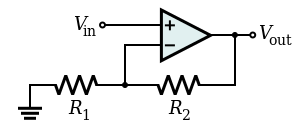
\includegraphics[width=.8\linewidth]{opAmp_nonInverting}
        \captionof{figure}{Non-Inverting Amplifier \cite{opAmpConfigurations}}
        \label{fig:opamp-non-inverting}
    \end{minipage}
    \begin{minipage}{.23\textwidth}
        \centering
        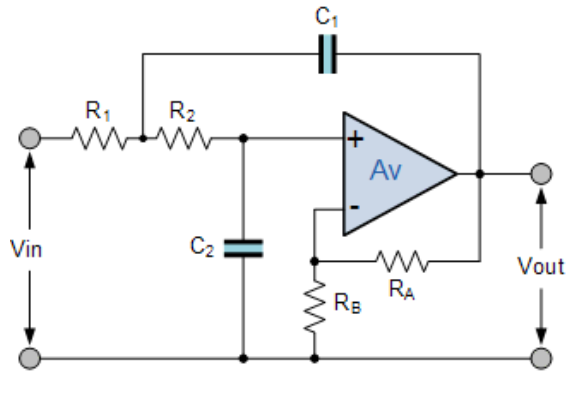
\includegraphics[width=0.8\linewidth]{opAmp_nonInverting_modified}
        \captionof{figure}{Modified Non-Inverting Amplifier \cite{opAmpSecondOrderFilters}}
        \label{fig:opamp-non-inverting-filter}
    \end{minipage}        
    \begin{minipage}{.23\textwidth}
        \centering
        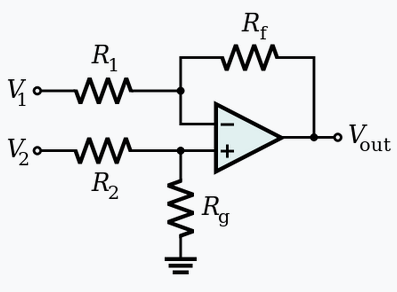
\includegraphics[width=.8\linewidth]{opAmp_differential}
        \captionof{figure}{Differential Amplifier \cite{opAmpConfigurations}}
        \label{fig:opamp-differential}
    \end{minipage}
    \begin{minipage}{.23\textwidth}
        \centering
        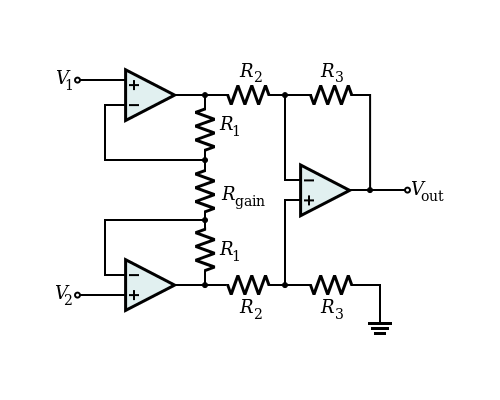
\includegraphics[width=0.9\linewidth]{opAmp_instrumentation}
        \captionof{figure}{Instrumentation Amplifier \cite{opAmpConfigurations}}
        \label{fig:opamp-instrumentation}
    \end{minipage}

\end{figure}

\pagebreak
\graphicspath{{content/1_literatureReview/figures/}}
\section{Current Sensing}

\subsection{Techniques}
Measurement techniques are usually either "invasive" or "non-invasive". Invasive techniques need to be built into the circuit directly and can have a significant affect
on its operation, whereas non-invasive techniques may be added after the initial circuit design e.g. by measurement of a conductor's magnetic field.
A list of a few of these techniques \cite{currentSenseMethods} include:
\begin{itemize}
    \item A current-sensing resistor in series, which uses Ohm's law with a voltage measurement to calculate current.
    \item Hall element sensors, which measure the potential difference created as a result of the main current's magnetic field bending another current left/right.
    \item Direct coil techniques, which make using of Faraday's law.
\end{itemize}

\begin{figure}[h!]
    \centering
    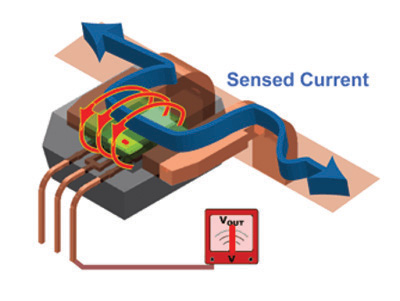
\includegraphics[width=.3\linewidth]{currentSensing_hall_effect}
    \captionof{figure}{Hall Effect Sensor Working Principle \cite{currentSenseHallEffect}}
    \label{fig:hall-effect}
  \end{figure}

\subsection{High-Side vs Low-Side}
This distinction refers to the placement of a current-sense element (e.g. resistor) relative to the load. For circuits which draw higher currents, high-side sensing can be used
(placing the resistor closer to the positive side of the voltage source) and is often more convenient. Low-side sensing, on the other hand, can potentially cause ground loop
issues \cite{currentSenseLowHighSide}, but has the ability to detect faults (e.g. short-circuits) earlier.

\subsection{AC, DC and Power Requirements}
As mentioned, there are various non-invasive and even wireless techniques used to measure current. Coil techniques make use of induction and therefore require AC to operate.
The Hall effect and sense resistors, on the other hand, may be used in the DC case. Wireless techniques have benefits over resistors in that they can be configured to draw much less power,
whereas sense resistors usually require high power handling capabilities as they pass all current drawn by the actual load through them.

\graphicspath{{content/figures/}}
\chapter{Detail design}\label{ch:detail_design}
%**********************************************
The following process details the design and calculations for the current sensor circuit. It provides insight into
what decisions were made, as well as the justifications behind them.

\section{Current sensor}\label{sec:current_sensor_design}
\subsubsection{Configuration}\label{sec:current_sensor_config}

The differential amplifier configuration will be used for this project for the following reasons:
\begin{itemize}
  \item The configuration is specifically designed to reject common-mode noise, which the non-inverting amp suffers from.
  \item Only 1 op-amp is needed.
  \item The design is relatively simple compared to the instrumentation amplifier.
\end{itemize}

However, a modified version with two extra capacitors will be used. Two capacitors will be added in parallel with $R_f$ and $R_g$ called $C_f$ and $C_g$ respectively. It is important that these capacitors have the same
value in order to preserve CMRR \cite{opAmpConfigurations}. It is likely, however, that one of these will be dominant due to differing resistor values, and therefore this design will only consider the filter to be first-order.
This is acceptable, however, due to the amplifier's noise-rejecting capabilities.

\subsubsection{Gain and Cutoff}\label{sec:current_sensor_circuit}
Before calculating component values, both the cutoff frequency of the RC filter, and the DC gain of the amplifier, need to be determined. The gain of the amplifier should be determined
such that, when the maximum current flows through the sense resistor, the maximum voltage is output.

First, the maximum current of the motor should be measured. This can be done by connecting the motor to a power supply (through an ammeter), stalling the motor, and reading the output current.
With a supply voltage of 6.4 V connected, the motor for this project read 740 mA, however different motors may read between 1 and 1.5 A. The average running current, however, is between 200 mA
and 300 mA. A value of $I_{max} = 1 A$ will therefore be chosen to allow for more headroom and a slightly lower gain.
Since a sense resistor of $\SI{10}{\milli\ohm}$ is to be used, the maximum voltage through this resistor will therefore be 8 mV. A gain of $\frac{3 V}{10 mV} = 300$ is therefore chosen.
Although this voltage level is small, it is expected, given that the resistance value is so small. It is also desirable, as it shows that the circuit is not "stealing" too much power from the motor itself.

The cutoff frequency $f_H$ should be selected such that the slew rate requirements are not affected, while still adequately filtering a 1 kHz noise signal. In order for the noise requirement
to be satisfied, the input signal must be attenuated by $20 \log{\frac{300 * 10 mV}{250 mV}} \approx 22 dB$. This means the cutoff should be around 100 Hz (a decade below 1 kHz).
Since the specification requires a change from 0.1 to $3 \times 0.9 = 2.7 V$ in less than 100 ms, the output should be capable of oscillating at $\frac{1}{50 ms} = 20 Hz$, which is below the designed cutoff.

Since input current of the circuit needs to be limited below 150 uA, high resistor values should be chosen:
\begin{itemize}
  \item Assuming $i_n = 0$, choose $\frac{V_{out(max)}}{R_1 + R_f} << 150 uA \therefore R_1 + R_f >> \SI{20}{\kilo\ohm}$. Choose $R_f = \SI{100}{\kilo\ohm}$.
  \item $G = \frac{R_f}{R_1} = 300 \therefore R_1 = \SI{330}{\ohm}$
  \item Choose $R_2 = R_1 = \SI{330}{\ohm}$ and $R_g = R_f = \SI{100}{\kilo\ohm}$ for differential symmetry.
  \item Since $R_{eq}$ of $C_f$ is $R_f$ and of $C_g$ is $R_g || R_2$, it is clear that $C_f$ is dominant, $\therefore C_f = \frac{1}{2 \pi \cdot R_f \cdot 100 Hz} \approx 15 nF$. Also set $C_g = 15nF$ for symmetry.
        It should be noted, however, that this technique (using time constants) is not always valid - especially in complex circuits such as these - and so these results should be checked using simulations.
\end{itemize}

\subsubsection{Circuit diagram}\label{sec:current_sensor_circuit}
The following figure details the final circuit design for the sensor and amplifier system.

\begin{figure}[h!]
  \centering
  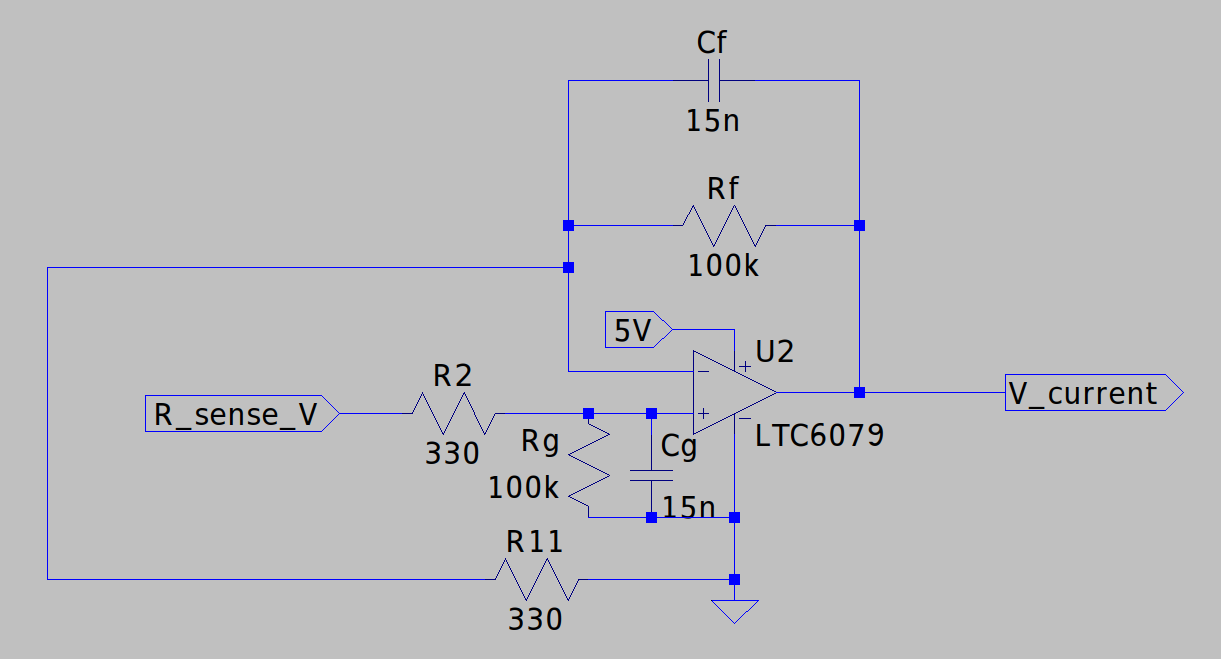
\includegraphics[width=.8\linewidth]{currentSensor_sim_circuit}
  \captionof{figure}{Circuit diagram of final configuration}  
  \label{fig:circuit-diagram}
\end{figure}

A single 5 V supply will be used. Although there are benefits to a dual rail supply, that would prove impractical in the context of the larger system.

\pagebreak

\graphicspath{{content/figures/}}
\chapter{Results}\label{ch:results}

\section{Current sensor}\label{sec:current_sensor_results}

\subsection{Simulation}

After running initial simulations, it was clear that the constant assumed in the design stage for the dominant capacitor $C_f$ was too high. The capacitor value was then experimentally
increased to 100nF where a satisfactory response which was reasonably below 250 mV (10-20\%) was obtained. This section details the rest of the results of these simulations.

\begin{figure}[h!]
   \centering
   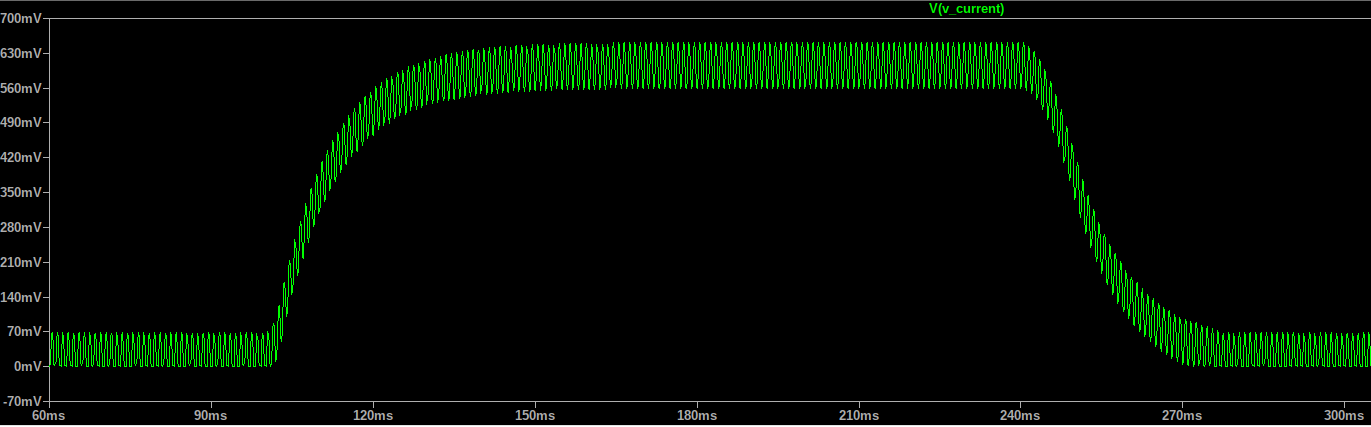
\includegraphics[width=.6\linewidth]{currentSensor_sim_stepResponse}
   \captionof{figure}{Amplifier output in response to step input}
   \label{fig:simulation response}
\end{figure}

\begin{figure}[h!]
   \centering
   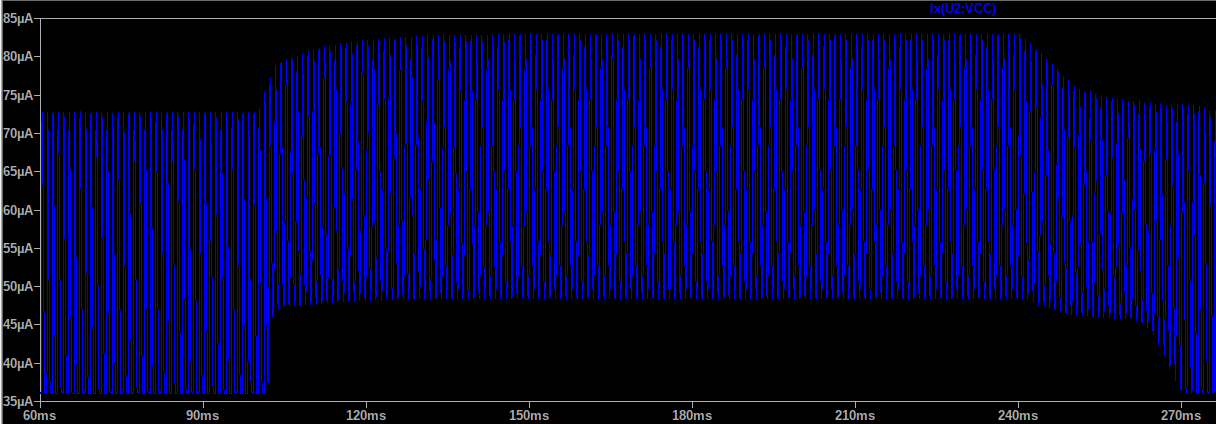
\includegraphics[width=.5\linewidth]{currentSensor_sim_currentDraw}
   \captionof{figure}{Current draw of op-amp}
   \label{fig:simulation_current}
\end{figure}

As can be seen, all specifications were adhered to:
\begin{itemize}
   \item The noise level at idle is well below the 250 mV requirement.
   \item The step response input changes 20-25 ms, which is below the 100 ms requirement.
   \item The power draw of the circuit (as measure at the positive terminal of the op-amp) is less than 85 uA, which is much less than the specified 150 uA.
\end{itemize}

Lastly, the input simulation parameters were modified during testing to analyze the various output voltages for different input currents. For input currents of 400mA, 500mA, 800mA and 1A,
the output voltages were 1.22V, 1.52, 2.43 and 3.024 V respectively. This matches perfectly with the initial design.

\subsection{Implementation}
Tests were conducted with a function generator to ensure the amplifier met specifications.

As can be seen in Figure \ref{fig:results_currentSensor_noise}, the amplifier noise requirement was satisfied. The input signal
(channel 1, bottom) is a \SI{10}{mV_{pp}} \SI{1}{kHz} sine wave with \SI{6}{mV} offset. It is required that a sinusoidal "noise" signal greater than this frequency
should not be amplified to more than \SI{250}{mV_{pp}}. An output of \SI{1.13}{V} - \SI{0.949}{V} = \SI{181}{mV} was obtained - within the threshold.

In Figure \ref{fig:results_currentSensor_response}, the amplifier's step response time was recorded as \SI{4.957}{ms}, which is much below the \SI{100}{ms} requirement.
This time is 4x better than the designed/simulated circuit, presumably due to the increased resistance value and other tolerances.

\begin{figure}[!h]
   \centering
   \begin{minipage}{0.45\textwidth}
      \centering
      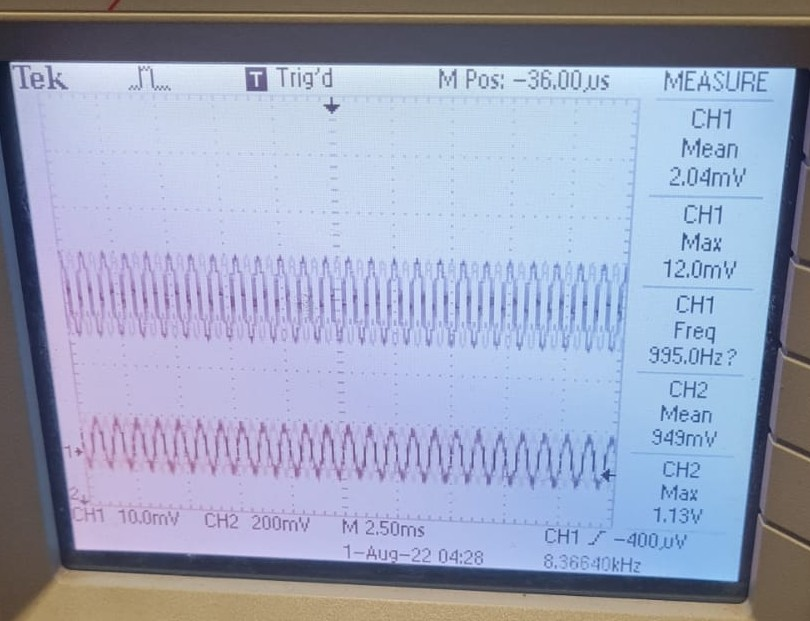
\includegraphics[width=0.7\linewidth]{currentSensor_impl_noise.jpeg}
      \captionof{figure}{Amplifier noise rejection}
      \label{fig:results_currentSensor_noise}
   \end{minipage}
   \begin{minipage}{0.45\textwidth}
      \centering
      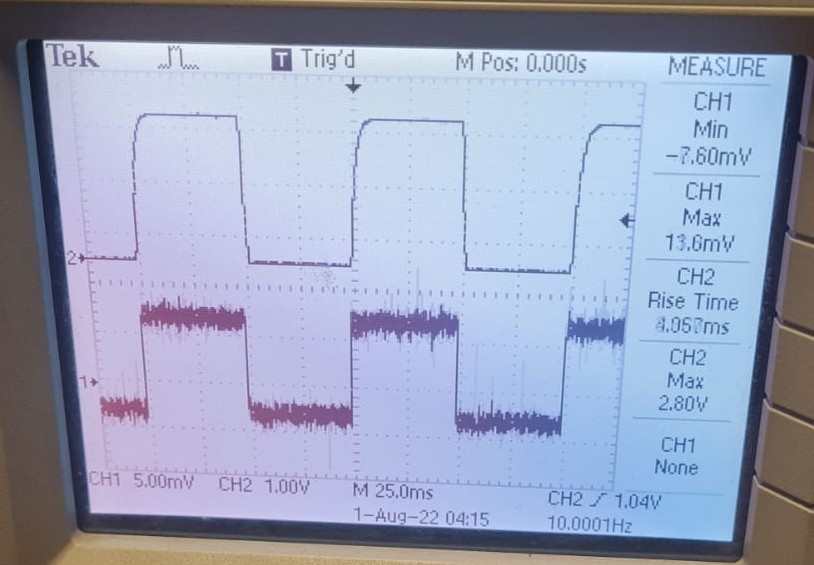
\includegraphics[width=0.7\linewidth]{currentSensor_impl_stepResponse.jpeg}
      \captionof{figure}{Amplifier response time}
      \label{fig:results_currentSensor_response}
   \end{minipage}
\end{figure}

Current measurements were then made with the motor connected, as visible in Table \ref{table:motor_currents}.
As can be analyzed, there is an offset voltage of \SI{0.42}{V} at the output. The actual gain can be calculated as e.g.
$\frac{\SI{1.42}{V} - \SI{0.42}{V}}{\SI{210}{\milli\ampere} * \SI{10}{\milli\ohm}}= 476 V/V$. With the \SI{120}{\kilo\ohm} resistor,
an ideal gain of $\frac{\SI{120}{\kilo\ohm}}{\SI{330}{\ohm}} = 363.6V/V$ was expected, however due to the nature of the circuit
(which contains 4 resistors) a tolerance of 10\% * 4 should be accounted for, which explains the higher gain.

\begin{table}[!h]
   \centering
   \begin{tabular}{ |c|c|c| }
      \hline
      \textbf{Motor Condition}         & \textbf{PSU Current (mA)}        & \textbf{Output  Voltage (V)}       \\ \hline
      Stall                            & 1200                             & 3.31                               \\ \hline
      Slight Load                      & 305                              & 1.96                               \\ \hline
      Free Running                     & 210                              & 1.42                               \\ \hline
      I = 150 mA                       & 150                              & 1.13                               \\ \hline
      I = 100 mA                       & 100                              & 0.91                               \\ \hline
      I = 50 mA                        & 50                               & 0.63                               \\ \hline
      I = 0 mA                         & 0                                & 0.42                               \\ \hline
   \end{tabular}\
   \caption{Measurements of Motor Current and Voltage}
   \label{table:motor_currents}   
\end{table}

\begin{figure}[!h]
   \centering
   \begin{minipage}{0.3\textwidth}
      \centering
      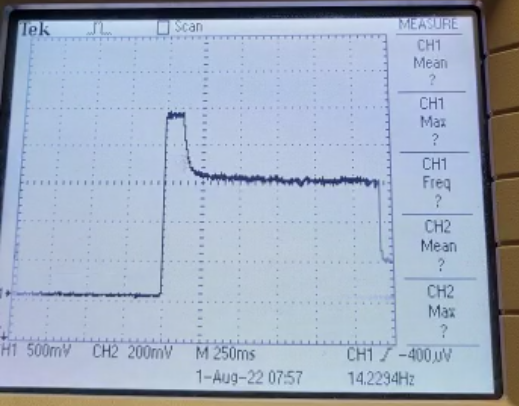
\includegraphics[width=0.7\linewidth]{currentSensor_impl_freeRunning}
      \captionof{figure}{0 A to free running}
   \end{minipage}
   \begin{minipage}{0.3\textwidth}
      \centering
      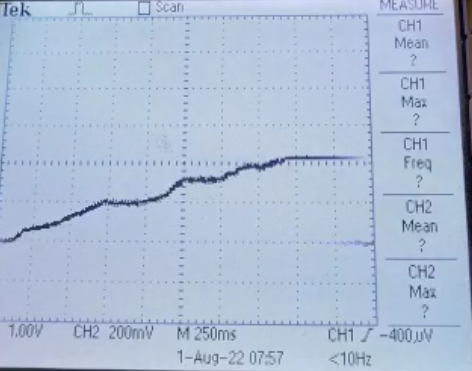
\includegraphics[width=0.7\linewidth]{currentSensor_impl_increasingLoad}
      \captionof{figure}{Increasing load}
   \end{minipage}
   \begin{minipage}{0.3\textwidth}
      \centering
      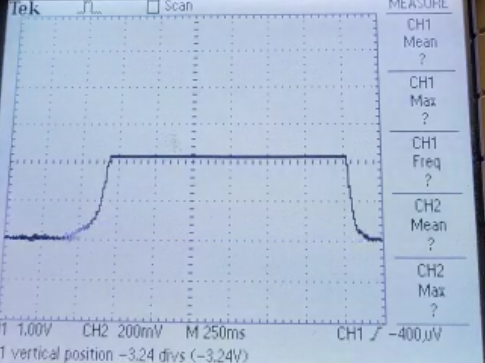
\includegraphics[width=0.7\linewidth]{currentSensor_impl_stall}
      \captionof{figure}{Free running to stall}
   \end{minipage}   
\end{figure}
\chapter{Physical implementation}\label{ch:implementation}

\graphicspath{{content/4_implementation/figures/}}
\section{Current sensor}\label{sec:current_sensor_physical}

The implementation of the circuit was different in two ways compared to the original design:
\begin{itemize}
   \item \SI{120}{\kilo\ohm} resistors were used instead of \SI{100}{\kilo\ohm}, as they were easier to obtain, and would only result in a
         slightly larger gain and lower cutoff.
   \item The amplifier circuit was powered with regulated \SI{3.3}{V}. This was done to protect the ESP's input pins by saturating the output
         when it would have been too large.
\end{itemize}

\begin{figure}[!htb]
  \centering
  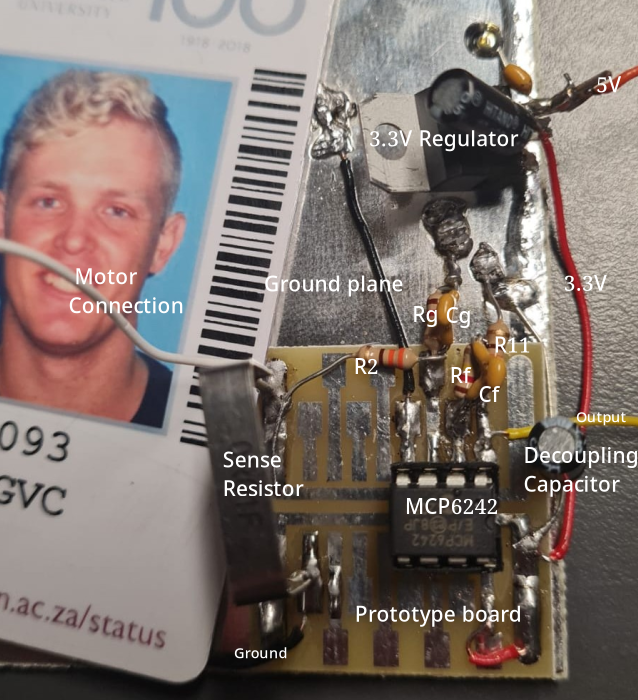
\includegraphics[width=0.75\textwidth]{currentSensor_impl_circuit}
  \caption{Final Circuit Implementation}
\end{figure}

% Bibliography
\bibliography{references}

% End matter
\appendix
\graphicspath{{endmatter/figures/}}
\chapter{Social contract}
\makeatletter\@mkboth{}{Appendix}\makeatother
\label{appen:social_contract}
     \begin{figure}[!htb]
     \centering
     	\fbox{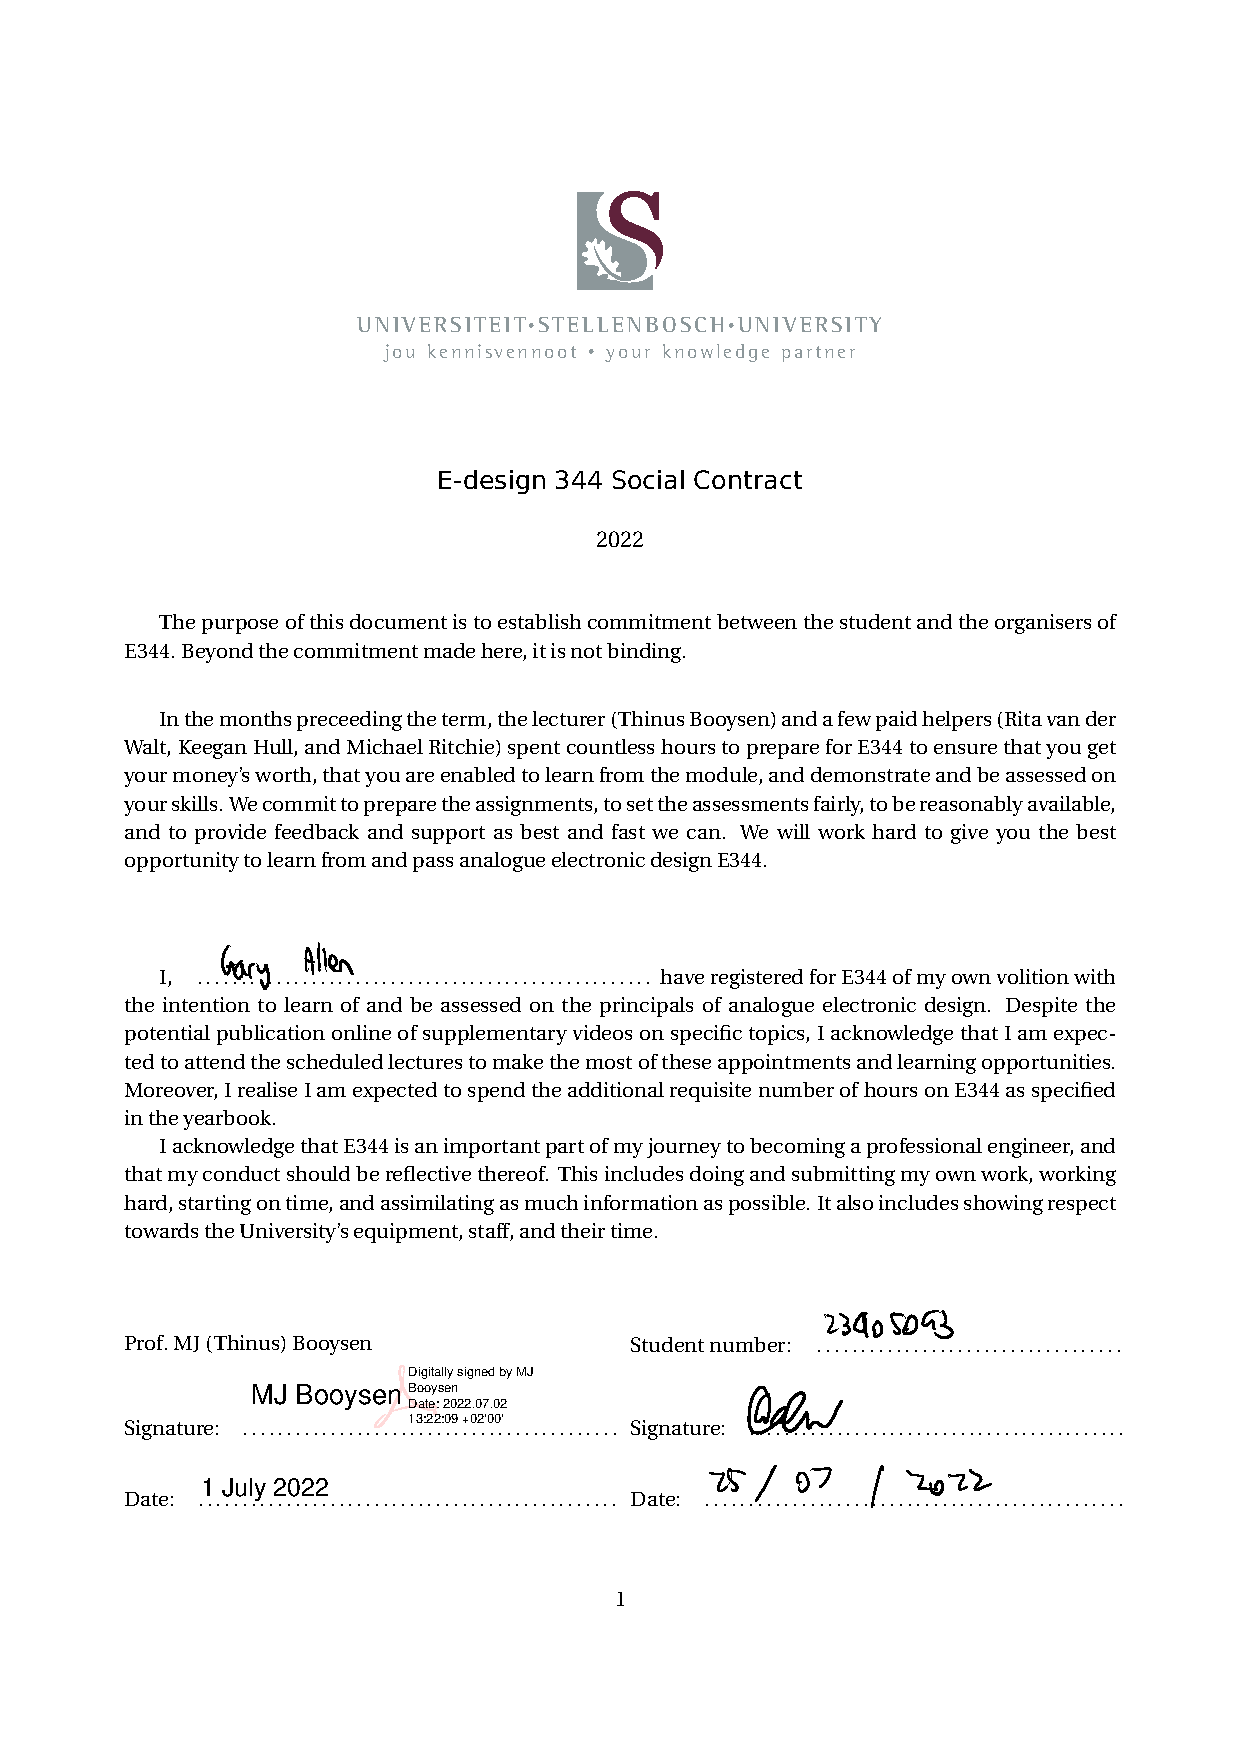
\includegraphics[width=0.8\linewidth]{SocialContract_signed.pdf}}
       \label{fig:social_contract}
	\end{figure}
\graphicspath{{endmatter/figures/}}
\chapter{GitHub Activity Heatmap}
\makeatletter\@mkboth{}{Appendix}\makeatother
\label{appen:github_heatmap}

     \begin{figure}[!htb]
     \centering
     	\fbox{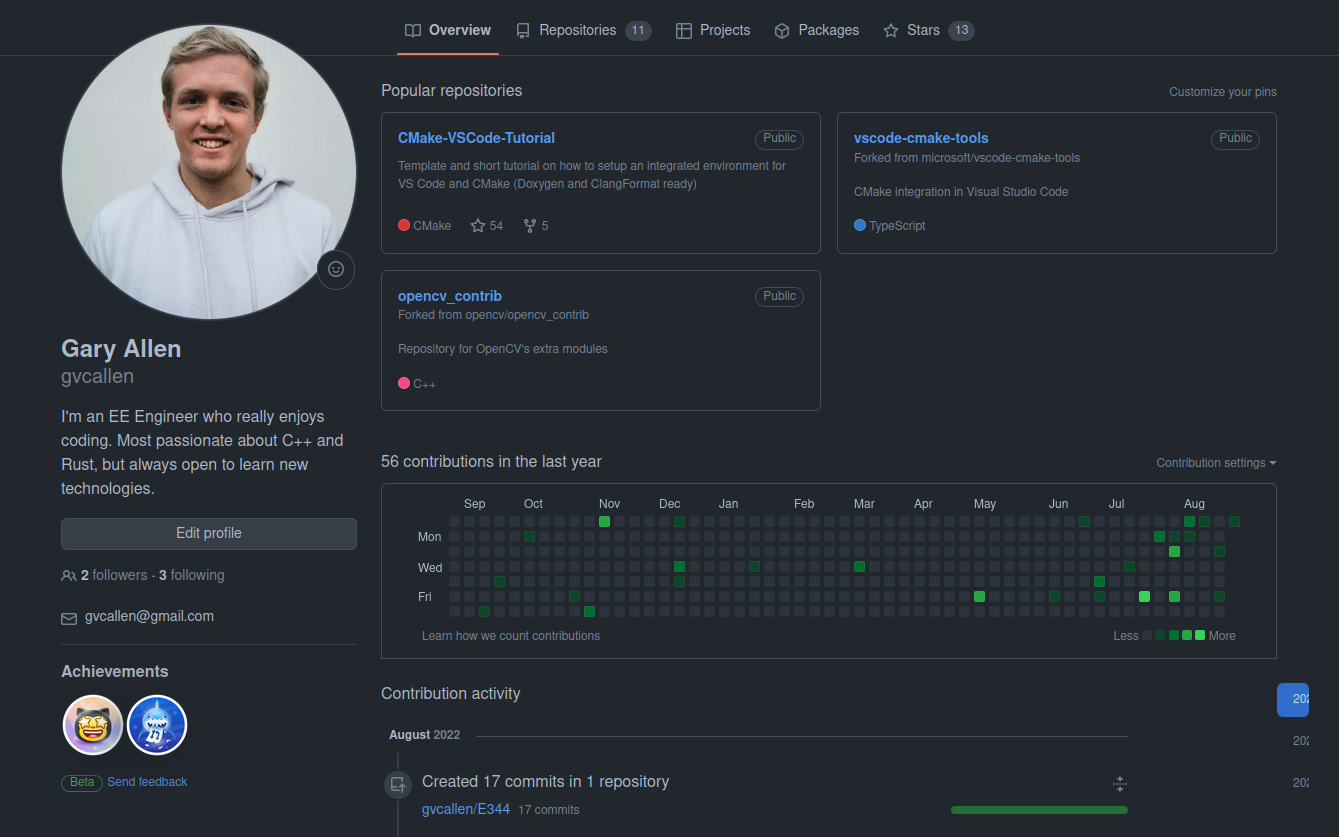
\includegraphics[width=1\linewidth]{GitHub.png}}
	\label{fig:github}
	\end{figure}

\end{document}